\documentclass[a4paper,12pt]{article} % добавить leqno в [] для нумерации слева
\usepackage[a4paper,top=1.3cm,bottom=2cm,left=1.5cm,right=1.5cm,marginparwidth=0.75cm]{geometry}
%%% Работа с русским языком
\usepackage{cmap}					% поиск в PDF
\usepackage{mathtext} 				% русские буквы в фомулах
\usepackage[T2A]{fontenc}			% кодировка
\usepackage[utf8]{inputenc}			% кодировка исходного текста
\usepackage[english,russian]{babel}	% локализация и переносы

\usepackage{graphicx}
\usepackage{mathtools}
\usepackage{wrapfig}
\usepackage{tabularx}
\usepackage{amssymb}
\usepackage{hyperref}
\usepackage[rgb]{xcolor}
\hypersetup{colorlinks=true,urlcolor=blue}
%% Шрифты
\usepackage{euscript}	 % Шрифт Евклид
\usepackage{amsmath}
\usepackage{mathtools}
%%% Заголовок
\author{Lokhmatov Arseniy}
\title{Лабораторная работа по общей физике}

\date{\today}
\begin{document}
\begin{titlepage}
    \newpage
    \begin{center}
    {\large МОСКОВСКИЙ ФИЗИКО-ТЕХНИЧЕСКИЙ ИНСТИТУТ (НАЦИОНАЛЬНЫЙ ИССЛЕДОВАТЕЛЬСКИЙ УНИВЕРСИТЕТ)}
    \vspace{1cm}

    {\largeФизтех-школа аэрокосмических технологий}
    \vspace{6em}
    \end{center}
    
    \vspace{1.2em}

    \begin{center}
    %\textsc{\textbf{}}
    \Large Лабораторная работа №3.3.4 \\
    Эффект Холла в полупроводниках
    \linebreak
    \end{center}
    
    \vspace{11em}
    
    \begin{flushright}
                       {\large Работу выполнил\\
                       Лохматов Арсений Игоревич\\
                       Б03-303 }
    \end{flushright}

    \vspace{\fill}

    \begin{center}
        
\includegraphics[width=0.2\linewidth]{dasr.png}
    \end{center}

    \begin{center}
    Долгопрудный, 2024
    \end{center}

    \end{titlepage}

\section{Теоретическая часть}

\paragraph{Цель работы:} измерение подвижности и концентрации носителей заряда в полупроводниках.


\paragraph{Оборудование:} электромагнит источником питания; вольтметр; амперметр; миллиамперметр; милливеберметр; источник питания; образцы легированного полупроводника.

\subsection{Теоретическая часть}

\par
В работе изучаются особенности проводимости полупроволников в геометрии \textit{мостика Холла}. Ток пропускается по плоской полупроводниковой пластинке, помещённой в перпендикулярное пластинке матнитное поле. Измеряется разность потенциалов между краями пластинки в поперечном к току направлении. По измерениям определяется \textit{констанка Холла}, тип проводимости (\textit{электронный} или \textit{дырочный}) и на основе соотношения ниже вычисляется концентрация основных носителей заряда. \par

\[ R_H = \frac{1}{nq}, \text{где } R_H - \textit{постоянная Холла}. \]

Электрическая схема установки для измерения ЭДС Холла представлена на рис. \ref{img1}.

\begin{figure}[h]
\begin{center}
		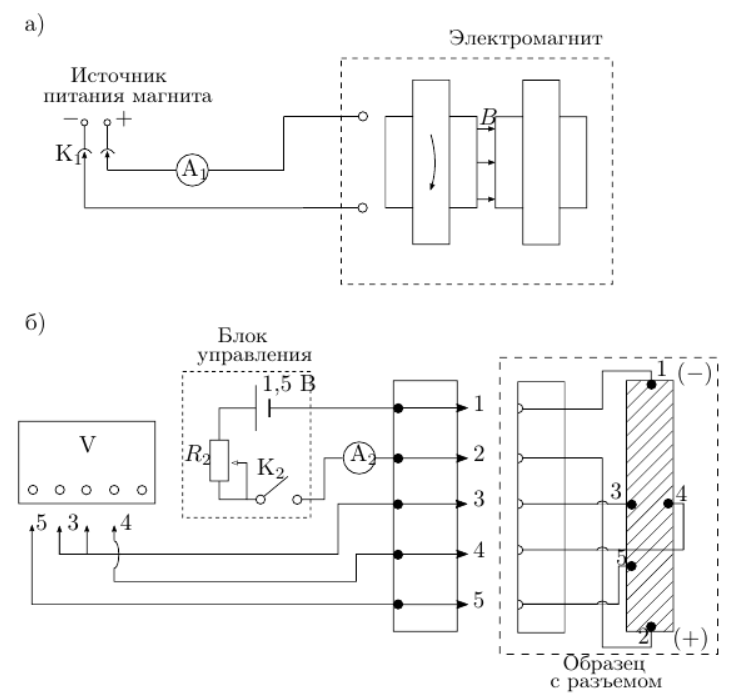
\includegraphics[width=12cm]{image_1_1.png}
\end{center}
	\caption{\textit{Схема установки для исследования эффекта Холла в полупроводниках}}
	\label{img1}
\end{figure}

В зазоре элетромагнита (рис. \ref{img1}а) создаётся постоянное магнитное поле, величину которого можно менять с помощью регулятора источника питания электромагнита. Ток питания электромагнита измеряется амперметром $A_1$. Напрвление тока в обмотках электромагнита меняется переключением разъёма $K_1$.\par

Градуировка электромагнита (связь тока с индукцией поля) проводится при помощи милливеберметра на основе датчика Холла.\par

Прямоугольный образец из легированного германия, смонтированный в специальном держателе (рис. \ref{img1}б), подключается к источнику питания ($1.5 B$). При замыкании ключа $K_2$ вдоль длинной стороны образца течёт ток, величина которого регулируется реостатом $R_2$ и измеряется миллиамперметром $A_2$.\par

В образце, помещённом в зазор электромагнита, между контактами $3$ и $4$ возникает разность потенциалов $U_{34}$, которая измеряется с помощью
вольтметра $V$.\par

Контакты 3 и 4 вследствие неточности подпайки могут лежать не на одной эквипотенциали. Тогда напряжение между ними связано не только с эффектом Холла, но и с омическим падением напряжения вдоль пластинки. Исключить этот эффект можно, изменяя направление магнитного поля, пронизывающего образец. При обращении поля ЭДС Холла меняет знак, а омическое падение напряжения остаётся неизменным. Поэтому ЭДС Холла $U_{\perp}$ может быть определена как половина алгебраической разности показаний вольтметра, полученных для двух противо-
положных направлений магнитного поля в зазоре: $U_{\perp} = \frac{1}{2}(U_{34}^{(+)} - U_{34}^{(-)})$).\par

Альтернативно можно исключить влияние омического падения напряжения, если при каждом значении тока через образец измерять напряжение между точками $3$ и $4$ в отсутствие магнитного поля. При фиксированном токе через образец это дополнительное к ЭДС Холла напряжение $U_0$ остаётся неизменным. От него следует (с учётом знака) отсчитывать величину ЭДС Холла:\par

\[ U_{\perp} = U_{34} - U_0. \]

При таком способе измерения нет необходимости проводить повторные измерения с противоположным направлением магнитного поля.\par

По знаку $U_{\perp}$ можно определить характер проводимости — электронный или дырочный. Для этого необходимо знать направление тока в образце и направление магнитного поля.\par

Измерив ток $I$ в образце и напряжение $U_{35}$ между контактами $3$ и $5$ в отсутствие магнитного поля, можно, зная параметры образца, рассчитать проводимость материала образца по формуле

\begin{equation}\label{1}
\sigma = \frac{IL_{35}}{U_{35}al},
\end{equation}

где $l$ — расстояние между контактами $3$ и $5$, $a$ — ширина образца, $h$ - его толщина.

\newpage
\section{Практическая часть}

\subsection{Приборные погрешности}

\[ \sigma_{a} = \pm 0.2 \%; \sigma_{v} = \pm 0.004 \%; \sigma_{vb} = \pm 1.5 \%. \]

\subsection{Градуировка электромагнита}

А можем далее устанавливать такое значение тока, при котором мы уже измерили индукцию магнитного поля. Мы воспользуемся вторым способом.

\subsection{Измерение ЭДС Холла}

Для разных значений $ I $ через образец снимем зависимость ЭДС Холла от тока $ I_\text{м} $ через электромагнит. Результаты измерений занесём в таблицу \ref{tab2}.

Последнее измерение было произведено при изменённой ориентации образца. Теперь вычислим значение $ \mathcal{E}_x $ по разности показаний вольтметра и сопоставим токи в электромагните с соответствующими значениями индукции магнитного поля. Полученные результаты занесём в таблицу \ref{tab3}.

По полученным данным построим графики зависимости $ \mathcal{E}_x(B) $ для различных значений $ I $.

\begin{figure}[h]
    \begin{center}
		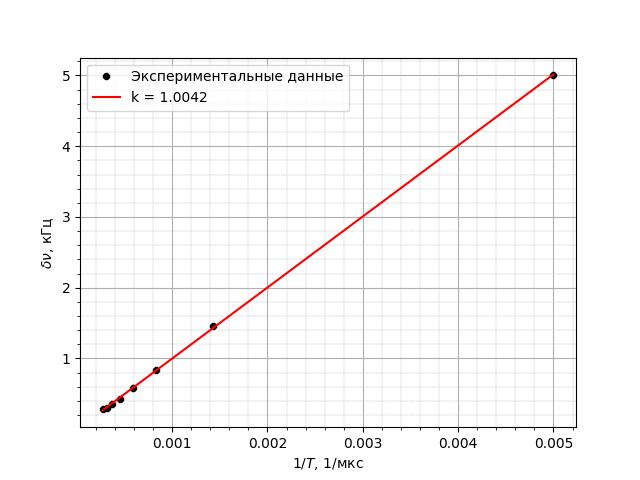
\includegraphics[width=18cm]{image2.jpg}
    \end{center}
	\caption{График зависимости $ \mathcal{E}_x(B) $}
\label{plot2}
\end{figure}

Аппроксимируем полученные данные зависимостями вида $  \mathcal{E}_x=K(I)B + C$ при помощи метода наименьшего квадрата (модуль $curvefit$ в Python). Результаты аппроксимации заносим в таблицу \ref{tab4}.

\begin{table}[h]
	\centering
	\begin{tabular}{|c|c|c|}
		\hline
		$ I $, мА & $ K(I)\cdot10^{-3} $, В/Тл & $ \sigma_{K(I)}\cdot10^{-3} $, В/Тл \\ \hline
		0.3  & 2.128 & 0.132   \\ \hline
		0.4  & 2.568 & 0.134   \\ \hline
		0.5  & 3.057 & 0.163   \\ \hline
		0.6  & 3.254 & 0.240   \\ \hline
		0.7  & 3.575 & 0.202   \\ \hline
		0.8  & 4.151 & 0.218   \\ \hline
		0.85 & 7.545 & 0.219   \\ \hline
	\end{tabular}
	\caption{Результаты аппроксимации}
	\label{tab4}
\end{table}

По этим данным построим график зависимости $ K(I) $ от $ I $.

\begin{figure}[h]
    \begin{center}
		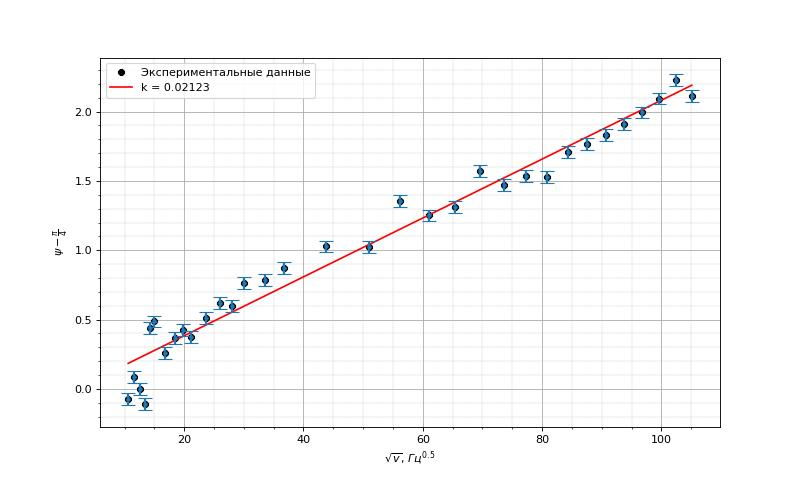
\includegraphics[width=14cm]{image3.jpg}
    \end{center}
	\caption{График зависимости $ K(I) $}
\label{plot3}
\end{figure}

Видим, что последняя точка явно выбивается из тренда, поэтому при аппроксимации её цчитывать не будем. Аппроксимируем зависимость прямой вида $ K=p\cdot I $. В итоге получаем 

\begin{equation}\label{9}
p = (5.51 \pm 0.25) \frac{\text{В}}{\text{Тл}\cdot\text{А}} \text{, }(\varepsilon = 4.54 \%).
\end{equation}

Тогда, согласно формуле

\[ \mathcal{E}_x = - \frac{IB}{nea} = - R_x \cdot \frac{IB}{a}, \]

$ R_x = pa $ -- коэффициент Холла, где $ a = 2 $ мм -- толщина исследуемого образца. После вычислений получаем:

\begin{equation}\label{10}
\boxed{R_x = (1.102\pm0.005) \cdot 10^{-3} \frac{\text{В}\cdot\text{м}}{\text{Тл}\cdot\text{А}} (\varepsilon = 0.45 \%)}.
\end{equation}

Отсюда найдём концентрацию носителей заряда согласно формуле, учитывая, у в нашем случае носителями заряда являются дырки. Погрешность определения концентрации есть погрешность определения постоянной Холла, так как считаем значение элементарного заряда известным.

\[ R_x=\frac{1}{ne}. \]

\begin{equation}\label{11}
\boxed{n = (543.38\pm2.45) \cdot 10^{19} \text{ м}^{-3}} \text{, }(\varepsilon = 0.45 \%). .
\end{equation}

\subsection{Расчёт удельной проводимости и подвижности}

По формуле \ref{1} рассчитаем удельную проводимость нашего образца. По результатам измерений $ U_{35} = 121.5 $ мВ, $ I = 0.89 $ мА, $ L_{35} = 15 $ мм и $ l = 8 $ мм, $ a = 2$ мм. Погрешность определения проводимости есть погрешность измерений силы тока амперметром ($ \sigma = 1\% $). В итоге получаем 

\begin{equation}\label{12}
\boxed{\sigma = (6.87\pm0.07)\text{ } (\text{Ом}\cdot\text{м})^{-1}}  \text{, }(\varepsilon = 1.02 \%). 
\end{equation}

Теперь, зная эти характеристики, можно рассчитать подвижность носителей заряда по следующей формуле:

\begin{equation}\label{13}
\mu=\frac{\sigma}{en}.
\end{equation}

В итоге получаем

\begin{equation}\label{14}
\boxed{\mu = (75.71\pm0.76) \text{ } \frac{\text{см}^2}{\text{В}\cdot\text{с}}}  \text{, }(\varepsilon = 1.01 \%). 
\end{equation}

\section{Вывод}

В ходе выполнения данной лабораторной работы был исследован эффект Холла в полупроводнике. Была определена постоянная Холла для исследуемого образца $ R_x = (1.102\pm0.005) \cdot 10^{-3} \text{ см}^{-3}/\text{Кл} $. Также была вычислена концентрация носителей заряда $ n = (543.38\pm2.45) \cdot 10^{19} \text{ м}^{-3}. $

По полярности вольтметра, полярности подключения источника тока и направлению тока в катушках была определён тип проводимости. Тип проводимости оказался дырочным.

Также была вычислена подвижность электронов в образце $ \mu = (75.71\pm0.76) \text{ } \text{см}^2/\text{В}\cdot\text{с} $. 


\begin{table}[h]
	\centering
	\begin{tabular}{l|cc|cc|cc|}
		\hline
		\multicolumn{1}{|c|}{$I$, мА}   & \multicolumn{2}{c|}{0,30} & 
            \multicolumn{2}{c|}{0,40} & \multicolumn{2}{c|}{0,50} \\ \hline
		\multicolumn{1}{|c|}{$U_0$, мВ} & \multicolumn{2}{c|}{-2.58} & 
            \multicolumn{2}{c|}{-3.16} & \multicolumn{2}{c|}{-3.87} \\ \hline
		\multicolumn{1}{c|}{} & \multicolumn{1}{c|}{$I_\text{м}$, А} & 
            $U$, мВ & \multicolumn{1}{c|}{$I_\text{м}$, А} & $U$, мВ &
            
            \multicolumn{1}{c|}{$I_\text{м}$, А} & $U$, мВ \\ \cline{2-7}
            
		\multicolumn{1}{c |}{} & \multicolumn{1}{c |}{ 0.1 } & -2.18 & 
            \multicolumn{1}{c |}{ 0.1 } &  -2.8  & \multicolumn{1}{c |}{ 0.1 } &  -3.44   \\ \cline{2 - 7}
            \multicolumn{1}{c |}{} & \multicolumn{1}{c |}{ 0.2 } & -1.81 & \multicolumn{1}{c |}{ 0.2 } &  -2.45  & \multicolumn{1}{c |}{ 0.2 } &  -3.03   \\ \cline{2 - 7}
            \multicolumn{1}{c |}{} & \multicolumn{1}{c |}{ 0.3 } & -1.55 & \multicolumn{1}{c |}{ 0.3 } &  -2.14  & \multicolumn{1}{c |}{ 0.3 } &  -2.63   \\ \cline{2 - 7}
            \multicolumn{1}{c |}{} & \multicolumn{1}{c |}{ 0.4 } & -1.34 & \multicolumn{1}{c |}{ 0.4 } &  -1.9  & \multicolumn{1}{c |}{ 0.4 } &  -2.36   \\ \cline{2 - 7}
            \multicolumn{1}{c |}{} & \multicolumn{1}{c |}{ 0.5 } & -1.15 & \multicolumn{1}{c |}{ 0.5 } &  -1.67  & \multicolumn{1}{c |}{ 0.5 } &  -2.09   \\ \cline{2 - 7}
            \multicolumn{1}{c |}{} & \multicolumn{1}{c |}{ 0.6 } & -1.02 & \multicolumn{1}{c |}{ 0.6 } &  -1.51  & \multicolumn{1}{c |}{ 0.6 } &  -1.89   \\ \cline{2 - 7}
            \multicolumn{1}{c |}{} & \multicolumn{1}{c |}{ 0.7 } & -0.89 & \multicolumn{1}{c |}{ 0.7 } &  -1.36  & \multicolumn{1}{c |}{ 0.7 } &  -1.72   \\ \cline{2 - 7}
            \multicolumn{1}{c |}{} & \multicolumn{1}{c |}{ 0.8 } & -0.78 & \multicolumn{1}{c |}{ 0.8 } &  -1.23  & \multicolumn{1}{c |}{ 0.8 } &  -1.56   \\ \cline{2 - 7}
            \multicolumn{1}{c |}{} & \multicolumn{1}{c |}{ 0.9 } & -0.69 & \multicolumn{1}{c |}{ 0.9 } &  -1.12  & \multicolumn{1}{c |}{ 0.9 } &  -1.44   \\ \cline{2 - 7}
            \multicolumn{1}{c |}{} & \multicolumn{1}{c |}{ 1.0 } & -0.62 & \multicolumn{1}{c |}{ 1.0 } &  -1.03  & \multicolumn{1}{c |}{ 1.0 } &  -1.31   \\ \cline{2 - 7}
            \multicolumn{1}{c |}{} & \multicolumn{1}{c |}{ 1.1 } & -0.55 & \multicolumn{1}{c |}{ 1.1 } &  -0.91  & \multicolumn{1}{c |}{ 1.1 } &  -1.2   \\ \cline{2 - 7}
            \multicolumn{1}{c |}{} & \multicolumn{1}{c |}{ 1.2 } & -0.48 & \multicolumn{1}{c |}{ 1.2 } &  -0.85  & \multicolumn{1}{c |}{ 1.2 } &  -1.09   \\ \cline{2 - 7}
            \multicolumn{1}{c |}{} & \multicolumn{1}{c |}{ 1.3 } & -0.41 & \multicolumn{1}{c |}{ 1.3 } &  -0.76  & \multicolumn{1}{c |}{ 1.3 } &  -1.0   \\ \cline{2 - 7}
            \multicolumn{1}{c |}{} & \multicolumn{1}{c |}{ 1.4 } & -0.36 & \multicolumn{1}{c |}{ 1.4 } &  -0.7  & \multicolumn{1}{c |}{ 1.4 } &  -0.93   \\ \cline{2 - 7}
            \multicolumn{1}{c |}{} & \multicolumn{1}{c |}{ 1.5 } & -0.31 & \multicolumn{1}{c |}{ 1.5 } &  -0.65  & \multicolumn{1}{c |}{ 1.5 } &  -0.85   \\ \cline{2 - 7}
            \multicolumn{1}{c |}{} & \multicolumn{1}{c |}{ 1.6 } & -0.28 & \multicolumn{1}{c |}{ 1.6 } &  -0.58  & \multicolumn{1}{c |}{ 1.6 } &  -0.81   \\ \cline{2 - 7}
            \multicolumn{1}{c |}{} & \multicolumn{1}{c |}{ 1.7 } & -0.26 & \multicolumn{1}{c |}{ 1.7 } &  -0.54  & \multicolumn{1}{c |}{ 1.7 } &  -0.76  \\ \cline{2 - 7}
            \multicolumn{1}{c |}{} & \multicolumn{1}{c |}{ 1.8 } & -0.23 & \multicolumn{1}{c |}{ 1.8 } &  -0.51  & \multicolumn{1}{c |}{ 1.8 } &  -0.71   \\ \cline{2 - 7}  \hline

		\multicolumn{1}{|c|}{$I$, мА} & \multicolumn{2}{c|}{0,60}          & \multicolumn{2}{c|}{0,70} & \multicolumn{2}{c|}{0,80} \\         \hline
  
		\multicolumn{1}{|c|}{$U_0$, мВ} & \multicolumn{2}{c|}{-4.62}       & \multicolumn{2}{c|}{-5.27} & \multicolumn{2}{c|}{-5.74} \\       \hline
  
		& \multicolumn{1}{c|}{$I_\text{м}$, А} & $U$, мВ &                 \multicolumn{1}{c|}{$I_\text{м}$, А} & $U$, мВ &    
            \multicolumn{1} {c|}{$I_\text{м}$, А} & $U$, мВ \\ \cline{2-7}
            
            \multicolumn{1}{c |}{} & \multicolumn{1}{c |}{ 0.1 } & -4.1 & \multicolumn{1}{c |}{ 0.1 } &  -4.5  & \multicolumn{1}{c |}{ 0.1 } &  -5.13   \\ \cline{2 - 7}
            \multicolumn{1}{c |}{} & \multicolumn{1}{c |}{ 0.2 } & -3.61 & \multicolumn{1}{c |}{ 0.2 } &  -4.03  & \multicolumn{1}{c |}{ 0.2 } &  -4.55   \\ \cline{2 - 7}
            \multicolumn{1}{c |}{} & \multicolumn{1}{c |}{ 0.3 } & -3.21 & \multicolumn{1}{c |}{ 0.3 } &  -3.56  & \multicolumn{1}{c |}{ 0.3 } &  -4.07   \\ \cline{2 - 7}
            \multicolumn{1}{c |}{} & \multicolumn{1}{c |}{ 0.4 } & -2.84 & \multicolumn{1}{c |}{ 0.4 } &  -3.14  & \multicolumn{1}{c |}{ 0.4 } &  -3.65   \\ \cline{2 - 7}
            \multicolumn{1}{c |}{} & \multicolumn{1}{c |}{ 0.5 } & -2.56 & \multicolumn{1}{c |}{ 0.5 } &  -2.89  & \multicolumn{1}{c |}{ 0.5 } &  -3.28   \\ \cline{2 - 7}
            \multicolumn{1}{c |}{} & \multicolumn{1}{c |}{ 0.6 } & -2.33 & \multicolumn{1}{c |}{ 0.6 } &  -2.64  & \multicolumn{1}{c |}{ 0.6 } &  -3.01   \\ \cline{2 - 7}
            \multicolumn{1}{c |}{} & \multicolumn{1}{c |}{ 0.7 } & -2.12 & \multicolumn{1}{c |}{ 0.7 } &  -2.46  & \multicolumn{1}{c |}{ 0.7 } &  -2.8   \\ \cline{2 - 7}
            \multicolumn{1}{c |}{} & \multicolumn{1}{c |}{ 0.8 } & -1.94 & \multicolumn{1}{c |}{ 0.8 } &  -2.28  & \multicolumn{1}{c |}{ 0.8 } &  -2.58   \\ \cline{2 - 7}
            \multicolumn{1}{c |}{} & \multicolumn{1}{c |}{ 0.9 } & -1.78 & \multicolumn{1}{c |}{ 0.9 } &  -2.13  & \multicolumn{1}{c |}{ 0.9 } &  -2.42   \\ \cline{2 - 7}
            \multicolumn{1}{c |}{} & \multicolumn{1}{c |}{ 1.0 } & -1.67 & \multicolumn{1}{c |}{ 1.0 } &  -1.99  & \multicolumn{1}{c |}{ 1.0 } &  -2.26   \\ \cline{2 - 7}
            \multicolumn{1}{c |}{} & \multicolumn{1}{c |}{ 1.1 } & -1.52 & \multicolumn{1}{c |}{ 1.1 } &  -1.88  & \multicolumn{1}{c |}{ 1.1 } &  -2.11   \\ \cline{2 - 7}
            \multicolumn{1}{c |}{} & \multicolumn{1}{c |}{ 1.2 } & -1.4 & \multicolumn{1}{c |}{ 1.2 } &  -1.73  & \multicolumn{1}{c |}{ 1.2 } &  -1.99   \\ \cline{2 - 7}
            \multicolumn{1}{c |}{} & \multicolumn{1}{c |}{ 1.3 } & -1.36 & \multicolumn{1}{c |}{ 1.3 } &  -1.63  & \multicolumn{1}{c |}{ 1.3 } &  -1.83   \\ \cline{2 - 7}
            \multicolumn{1}{c |}{} & \multicolumn{1}{c |}{ 1.4 } & -1.31 & \multicolumn{1}{c |}{ 1.4 } &  -1.55  & \multicolumn{1}{c |}{ 1.4 } &  -1.73   \\ \cline{2 - 7}
            \multicolumn{1}{c |}{} & \multicolumn{1}{c |}{ 1.5 } & -1.24 & \multicolumn{1}{c |}{ 1.5 } &  -1.47  & \multicolumn{1}{c |}{ 1.5 } &  -1.62   \\ \cline{2 - 7}
            \multicolumn{1}{c |}{} & \multicolumn{1}{c |}{ 1.6 } & -1.19 & \multicolumn{1}{c |}{ 1.6 } &  -1.4  & \multicolumn{1}{c |}{ 1.6 } &  -1.54   \\ \cline{2 - 7}
            \multicolumn{1}{c |}{} & \multicolumn{1}{c |}{ 1.7 } & -1.5 & \multicolumn{1}{c |}{ 1.7 } &  -1.33  & \multicolumn{1}{c |}{ 1.7 } &  -1.47   \\ \cline{2 - 7}
            \multicolumn{1}{c |}{} & \multicolumn{1}{c |}{ 1.8 } & -1.12 & \multicolumn{1}{c |}{ 1.8 } &  -1.28  & \multicolumn{1}{c |}{ 1.8 } &  -1.39   \\ \cline{2 - 7} \hline

		\multicolumn{1}{|c|}{$I$, мА} & \multicolumn{2}{c}{} &             \multicolumn{2}{c}{0.85 (flip)} & \multicolumn{2}{c|}{}            \\ \hline
  
		\multicolumn{1}{|c|}{$U_0$, мВ} & \multicolumn{2}{c}{}             & \multicolumn{2}{c}{-6.53 (flip)} & \multicolumn{2}{c|}{} \\  
            \hline
            
		& \multicolumn{1}{c|}{$I_\text{м}$, А} & $U$, мВ &    
            \multicolumn{1}{c|}{$I_\text{м}$, А} & $U$, мВ & \multicolumn{1}{c|}{$I_\text{м}$, А} & $U$, мВ \\ \cline{2-7}
  
            \multicolumn{1}{c |}{} & \multicolumn{1}{c |}{ 0.1 } & -7.22 & \multicolumn{1}{c |}{ 0.7 } &  -10.51  & \multicolumn{1}{c |}{ 1.3 } &  -12.97   \\ \cline{2 - 7}
            \multicolumn{1}{c |}{} & \multicolumn{1}{c |}{ 0.2 } & -7.91 & \multicolumn{1}{c |}{ 0.8 } &  -10.89  & \multicolumn{1}{c |}{ 1.4 } &  -13.12   \\ \cline{2 - 7}
            \multicolumn{1}{c |}{} & \multicolumn{1}{c |}{ 0.3 } & -8.55 & \multicolumn{1}{c |}{ 0.9 } &  -11.08  & \multicolumn{1}{c |}{ 1.5 } &  -13.21   \\ \cline{2 - 7}
            \multicolumn{1}{c |}{} & \multicolumn{1}{c |}{ 0.4 } & -9.16 & \multicolumn{1}{c |}{ 1.0 } &  -11.4  & \multicolumn{1}{c |}{ 1.6 } &  -13.32   \\ \cline{2 - 7}
            \multicolumn{1}{c |}{} & \multicolumn{1}{c |}{ 0.5 } & -9.67 & \multicolumn{1}{c |}{ 1.1 } &  -11.71  & \multicolumn{1}{c |}{ 1.7 } &  -13.37   \\ \cline{2 - 7}
            \multicolumn{1}{c |}{} & \multicolumn{1}{c |}{ 0.6 } & -10.11 & \multicolumn{1}{c |}{ 1.2 } &  -11.96  & \multicolumn{1}{c |}{ 1.8 } &  -13.4   \\ \cline{2 - 7}
	\end{tabular}
	\caption{Измерение ЭДС Холла}
	\label{tab2}
\end{table}

\begin{table}[h]
	\centering
	\begin{tabular}{l|cc|cc|cc|}
		\hline
		\multicolumn{1}{|c|}{$I$, мА}   & \multicolumn{2}{c|}{0,30} & 
            \multicolumn{2}{c|}{0,40} & \multicolumn{2}{c|}{0,50} \\ \hline
		
		\multicolumn{1}{c|}{} & \multicolumn{1}{c|}{$B$, мТл} & 
            $\mathcal{E}_x$, мВ &
            \multicolumn{1}{c|}{$B$, мТл} & $\mathcal{E}_x$, мВ & 
            \multicolumn{1}{c|}{$B$, мТл} & $\mathcal{E}_x$, мВ \\ \cline{2-7}
            
		\multicolumn{1}{c |}{} & \multicolumn{1}{c |}{ 74.667 } & 0.4 
             & \multicolumn{1}{c |}{ 74.667 } &  0.36  & \multicolumn{1}{c |}{ 74.667 } &  0.43   \\ \cline{2 - 7}
            \multicolumn{1}{c |}{} & \multicolumn{1}{c |}{ 133.333 } & 0.77 & \multicolumn{1}{c |}{ 133.333 } &  0.71  & \multicolumn{1}{c |}{ 133.333 } &  0.84   \\ \cline{2 - 7}
            \multicolumn{1}{c |}{} & \multicolumn{1}{c |}{ 186.667 } & 1.03 & \multicolumn{1}{c |}{ 186.667 } &  1.02  & \multicolumn{1}{c |}{ 186.667 } &  1.24   \\ \cline{2 - 7}
            \multicolumn{1}{c |}{} & \multicolumn{1}{c |}{ 246.667 } & 1.24 & \multicolumn{1}{c |}{ 246.667 } &  1.26  & \multicolumn{1}{c |}{ 246.667 } &  1.51   \\ \cline{2 - 7}
            \multicolumn{1}{c |}{} & \multicolumn{1}{c |}{ 306.667 } & 1.43 & \multicolumn{1}{c |}{ 306.667 } &  1.49  & \multicolumn{1}{c |}{ 306.667 } &  1.78   \\ \cline{2 - 7}
            \multicolumn{1}{c |}{} & \multicolumn{1}{c |}{ 377.333 } & 1.56 & \multicolumn{1}{c |}{ 377.333 } &  1.65  & \multicolumn{1}{c |}{ 377.333 } &  1.98   \\ \cline{2 - 7}
            \multicolumn{1}{c |}{} & \multicolumn{1}{c |}{ 426.667 } & 1.69 & \multicolumn{1}{c |}{ 426.667 } &  1.8  & \multicolumn{1}{c |}{ 426.667 } &  2.15   \\ \cline{2 - 7}
            \multicolumn{1}{c |}{} & \multicolumn{1}{c |}{ 484.0 } & 1.8 & \multicolumn{1}{c |}{ 484.0 } &  1.93  & \multicolumn{1}{c |}{ 484.0 } &  2.31   \\ \cline{2 - 7}
            \multicolumn{1}{c |}{} & \multicolumn{1}{c |}{ 540.0 } & 1.89 & \multicolumn{1}{c |}{ 540.0 } &  2.04  & \multicolumn{1}{c |}{ 540.0 } &  2.43   \\ \cline{2 - 7}
            \multicolumn{1}{c |}{} & \multicolumn{1}{c |}{ 588.0 } & 1.96 & \multicolumn{1}{c |}{ 588.0 } &  2.13  & \multicolumn{1}{c |}{ 588.0 } &  2.56   \\ \cline{2 - 7}
            \multicolumn{1}{c |}{} & \multicolumn{1}{c |}{ 645.333 } & 2.03 & \multicolumn{1}{c |}{ 645.333 } &  2.25  & \multicolumn{1}{c |}{ 645.333 } &  2.67   \\ \cline{2 - 7}
            \multicolumn{1}{c |}{} & \multicolumn{1}{c |}{ 693.333 } & 2.1 & \multicolumn{1}{c |}{ 693.333 } &  2.31  & \multicolumn{1}{c |}{ 693.333 } &  2.78   \\ \cline{2 - 7}
            \multicolumn{1}{c |}{} & \multicolumn{1}{c |}{ 732.0 } & 2.17 & \multicolumn{1}{c |}{ 732.0 } &  2.4  & \multicolumn{1}{c |}{ 732.0 } &  2.87   \\ \cline{2 - 7}
            \multicolumn{1}{c |}{} & \multicolumn{1}{c |}{ 773.333 } & 2.22 & \multicolumn{1}{c |}{ 773.333 } &  2.46  & \multicolumn{1}{c |}{ 773.333 } &  2.94   \\ \cline{2 - 7}
            \multicolumn{1}{c |}{} & \multicolumn{1}{c |}{ 800.0 } & 2.27 & \multicolumn{1}{c |}{ 800.0 } &  2.51  & \multicolumn{1}{c |}{ 800.0 } &  3.02   \\ \cline{2 - 7}
            \multicolumn{1}{c |}{} & \multicolumn{1}{c |}{ 825.333 } & 2.3 & \multicolumn{1}{c |}{ 825.333 } &  2.58  & \multicolumn{1}{c |}{ 825.333 } &  3.06   \\ \cline{2 - 7}
            \multicolumn{1}{c |}{} & \multicolumn{1}{c |}{ 853.333 } & 2.32 & \multicolumn{1}{c |}{ 853.333 } &  2.62  & \multicolumn{1}{c |}{ 853.333 } &  3.11   \\ \cline{2 - 7}
            \multicolumn{1}{c |}{} & \multicolumn{1}{c |}{ 866.667 } & 2.35 & \multicolumn{1}{c |}{ 866.667 } &  2.65  & \multicolumn{1}{c |}{ 866.667 } &  3.16   \\ \cline{2 - 7} \hline

            \multicolumn{1}{|c|}{$I$, мА}   & \multicolumn{2}{c|}{0,60} & 
            \multicolumn{2}{c|}{0,70} & \multicolumn{2}{c|}{0,80} \\ \hline
		
		\multicolumn{1}{c|}{} & \multicolumn{1}{c|}{$B$, мТл} & 
            $\mathcal{E}_x$, мВ &
            \multicolumn{1}{c|}{$B$, мТл} & $\mathcal{E}_x$, мВ & 
            \multicolumn{1}{c|}{$B$, мТл} & $\mathcal{E}_x$, мВ \\ \cline{2-7}

            \multicolumn{1}{c |}{} & \multicolumn{1}{c |}{ 74.667 } & 0.52 & \multicolumn{1}{c |}{ 74.667 } &  0.77  & \multicolumn{1}{c |}{ 74.667 } &  0.61   \\ \cline{2 - 7}
            \multicolumn{1}{c |}{} & \multicolumn{1}{c |}{ 133.333 } & 1.01 & \multicolumn{1}{c |}{ 133.333 } &  1.24  & \multicolumn{1}{c |}{ 133.333 } &  1.19   \\ \cline{2 - 7}
            \multicolumn{1}{c |}{} & \multicolumn{1}{c |}{ 186.667 } & 1.41 & \multicolumn{1}{c |}{ 186.667 } &  1.71  & \multicolumn{1}{c |}{ 186.667 } &  1.67   \\ \cline{2 - 7}
            \multicolumn{1}{c |}{} & \multicolumn{1}{c |}{ 246.667 } & 1.78 & \multicolumn{1}{c |}{ 246.667 } &  2.13  & \multicolumn{1}{c |}{ 246.667 } &  2.09   \\ \cline{2 - 7}
            \multicolumn{1}{c |}{} & \multicolumn{1}{c |}{ 306.667 } & 2.06 & \multicolumn{1}{c |}{ 306.667 } &  2.38  & \multicolumn{1}{c |}{ 306.667 } &  2.46   \\ \cline{2 - 7}
            \multicolumn{1}{c |}{} & \multicolumn{1}{c |}{ 377.333 } & 2.29 & \multicolumn{1}{c |}{ 377.333 } &  2.63  & \multicolumn{1}{c |}{ 377.333 } &  2.73   \\ \cline{2 - 7}
            \multicolumn{1}{c |}{} & \multicolumn{1}{c |}{ 426.667 } & 2.5 & \multicolumn{1}{c |}{ 426.667 } &  2.81  & \multicolumn{1}{c |}{ 426.667 } &  2.94   \\ \cline{2 - 7}
            \multicolumn{1}{c |}{} & \multicolumn{1}{c |}{ 484.0 } & 2.68 & \multicolumn{1}{c |}{ 484.0 } &  2.99  & \multicolumn{1}{c |}{ 484.0 } &  3.16   \\ \cline{2 - 7}
            \multicolumn{1}{c |}{} & \multicolumn{1}{c |}{ 540.0 } & 2.84 & \multicolumn{1}{c |}{ 540.0 } &  3.14  & \multicolumn{1}{c |}{ 540.0 } &  3.32   \\ \cline{2 - 7}
            \multicolumn{1}{c |}{} & \multicolumn{1}{c |}{ 588.0 } & 2.95 & \multicolumn{1}{c |}{ 588.0 } &  3.28  & \multicolumn{1}{c |}{ 588.0 } &  3.48   \\ \cline{2 - 7}
            \multicolumn{1}{c |}{} & \multicolumn{1}{c |}{ 645.333 } & 3.1 & \multicolumn{1}{c |}{ 645.333 } &  3.39  & \multicolumn{1}{c |}{ 645.333 } &  3.63   \\ \cline{2 - 7}
            \multicolumn{1}{c |}{} & \multicolumn{1}{c |}{ 693.333 } & 3.22 & \multicolumn{1}{c |}{ 693.333 } &  3.54  & \multicolumn{1}{c |}{ 693.333 } &  3.75   \\ \cline{2 - 7}
            \multicolumn{1}{c |}{} & \multicolumn{1}{c |}{ 732.0 } & 3.26 & \multicolumn{1}{c |}{ 732.0 } &  3.64  & \multicolumn{1}{c |}{ 732.0 } &  3.91   \\ \cline{2 - 7}
            \multicolumn{1}{c |}{} & \multicolumn{1}{c |}{ 773.333 } & 3.31 & \multicolumn{1}{c |}{ 773.333 } &  3.72  & \multicolumn{1}{c |}{ 773.333 } &  4.01   \\ \cline{2 - 7}
            \multicolumn{1}{c |}{} & \multicolumn{1}{c |}{ 800.0 } & 3.38 & \multicolumn{1}{c |}{ 800.0 } &  3.8  & \multicolumn{1}{c |}{ 800.0 } &  4.12   \\ \cline{2 - 7}
            \multicolumn{1}{c |}{} & \multicolumn{1}{c |}{ 825.333 } & 3.43 & \multicolumn{1}{c |}{ 825.333 } &  3.87  & \multicolumn{1}{c |}{ 825.333 } &  4.2   \\ \cline{2 - 7}
            \multicolumn{1}{c |}{} & \multicolumn{1}{c |}{ 853.333 } & 3.12 & \multicolumn{1}{c |}{ 853.333 } &  3.94  & \multicolumn{1}{c |}{ 853.333 } &  4.27   \\ \cline{2 - 7}
            \multicolumn{1}{c |}{} & \multicolumn{1}{c |}{ 866.667 } & 3.5 & \multicolumn{1}{c |}{ 866.667 } &  3.99  & \multicolumn{1}{c |}{ 866.667 } &  4.35   \\ \cline{2 - 7} \hline

            \multicolumn{1}{|c|}{$I$, мА} & \multicolumn{2}{c}{} & \multicolumn{2}{c}{0.85 (flip)} & \multicolumn{2}{c|}{} \\  
            \hline
		\multicolumn{1}{c|}{} & \multicolumn{1}{c|}{$B$, мТл} & 
            $\mathcal{E}_x$, мВ &
            \multicolumn{1}{c|}{$B$, мТл} & $\mathcal{E}_x$, мВ & 
            \multicolumn{1}{c|}{$B$, мТл} & $\mathcal{E}_x$, мВ \\ \cline{2-7}

            \multicolumn{1}{c |}{} & \multicolumn{1}{c |}{ 74.667 } & -0.69 & \multicolumn{1}{c |}{ 426.667 } &  -3.98  & \multicolumn{1}{c |}{ 732.0 } &  -6.44   \\ \cline{2 - 7}
            \multicolumn{1}{c |}{} & \multicolumn{1}{c |}{ 133.333 } & -1.38 & \multicolumn{1}{c |}{ 484.0 } &  -4.36  & \multicolumn{1}{c |}{ 773.333 } &  -6.59   \\ \cline{2 - 7}
            \multicolumn{1}{c |}{} & \multicolumn{1}{c |}{ 186.667 } & -2.02 & \multicolumn{1}{c |}{ 540.0 } &  -4.55  & \multicolumn{1}{c |}{ 800.0 } &  -6.68   \\ \cline{2 - 7}
            \multicolumn{1}{c |}{} & \multicolumn{1}{c |}{ 246.667 } & -2.63 & \multicolumn{1}{c |}{ 588.0 } &  -4.87  & \multicolumn{1}{c |}{ 825.333 } &  -6.79   \\ \cline{2 - 7}
            \multicolumn{1}{c |}{} & \multicolumn{1}{c |}{ 306.667 } & -3.14 & \multicolumn{1}{c |}{ 645.333 } &  -5.18  & \multicolumn{1}{c |}{ 853.333 } &  -6.84   \\ \cline{2 - 7}
            \multicolumn{1}{c |}{} & \multicolumn{1}{c |}{ 377.333 } & -3.58 & \multicolumn{1}{c |}{ 693.333 } &  -5.43  & \multicolumn{1}{c |}{ 866.667 } &  -6.87   \\ \cline{2 - 7}

	\end{tabular}
	\caption{Результаты вычислений}
	\label{tab3}
\end{table}

\newpage

\subsection{Приложение}

\begin{figure}[h]
    \begin{minipage}[h]{0.5\linewidth}
        \center{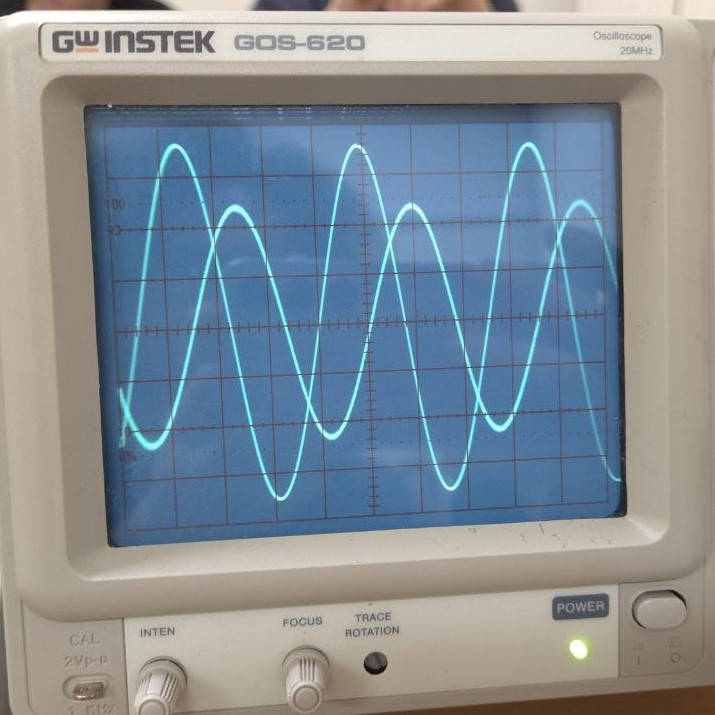
\includegraphics[width=0.8\linewidth]{1.jpg}}
    \end{minipage}
    \begin{minipage}[h]{0.5\linewidth}
        \center{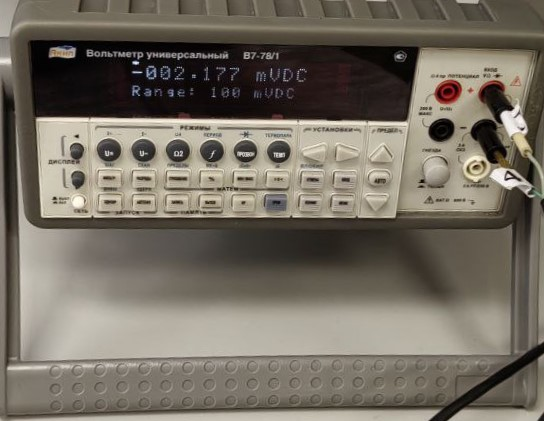
\includegraphics[width=0.8\linewidth]{2.jpg}}
    \end{minipage}
    \begin{minipage}[h]{0.5\linewidth}
        \center{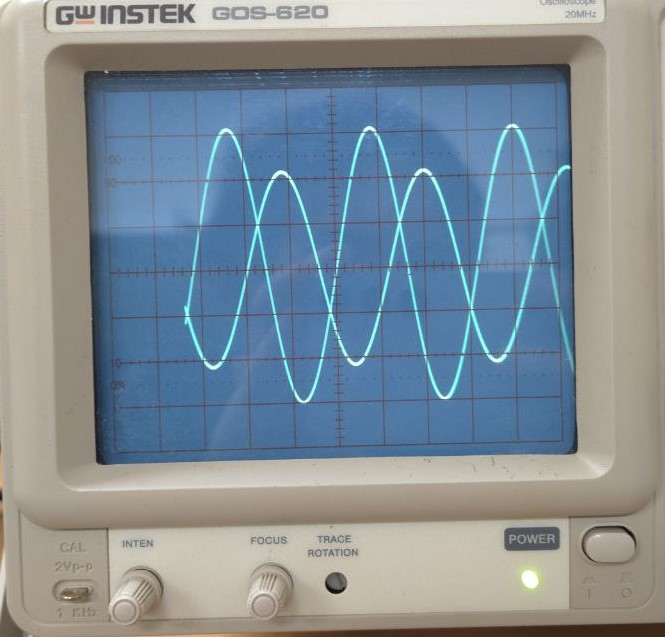
\includegraphics[width=0.8\linewidth]{3.jpg}}
    \end{minipage}
    \begin{minipage}[h]{0.5\linewidth}
        \center{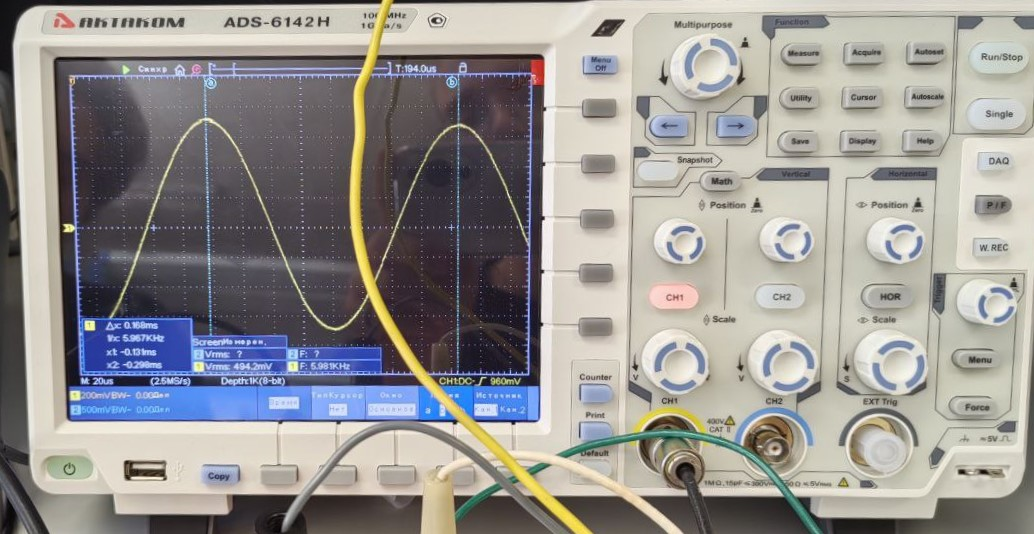
\includegraphics[width=0.8\linewidth]{4.jpg}}
    \end{minipage}
\end{figure}

\end{document}